%!TEX root = ../main.tex

\chapter{E2E simulation of NR in NTN scenario}
\label{chp:scheduling_problems}

Given the absence of a tool to properly simulate the behavior of the \ac{NR} stack in a non-terrestrial scenario, the first objective of this thesis is to design and implement some modifications to the protocol stack in order to make it work with long propagation delays. The current codebase of ns3-mmWave and ns3-ntn modules only provide separate implementations of the \ac{NR} stack and the non-terrestrial channel model.

The objective of obtaining a base support that permitted \ac{NTN} \ac{NR} simulation was achieved by devising a \ac{NTN} test scenario where we implemented the \ac{NR} stack, launching simulations and examining the results. Each unexpected behavior was documented, analyzed and solved proposing original solutions. Such work was necessary since the current state of the art regarding network simulators is still lacking proper support for the scenario we meant to investigate.

After describing the network topology and scenario that we implemented in the simulator, this chapter focuses on the problems that hampered the ability to correctly send and receive packets. Since many of them involved the scheduler, a brief introduction about the scheduler and its working principles is presented, then each implemented solution is detailed.

\section{Implemented scenario}

This section aims at describing the reference scenario that was implemented in the ns-3 simulator in order to test the \ac{NR} protocol suite in a non-terrestrial communication setting.

\subsection{Network topology}
To conduct the various simulation campaigns, ensuring the reproducibility and the comparability of the obtained results, a reference network topology has been made, and the parameters specified by \ac{3GPP} have been used.

\begin{figure}[ht]
    \centering
    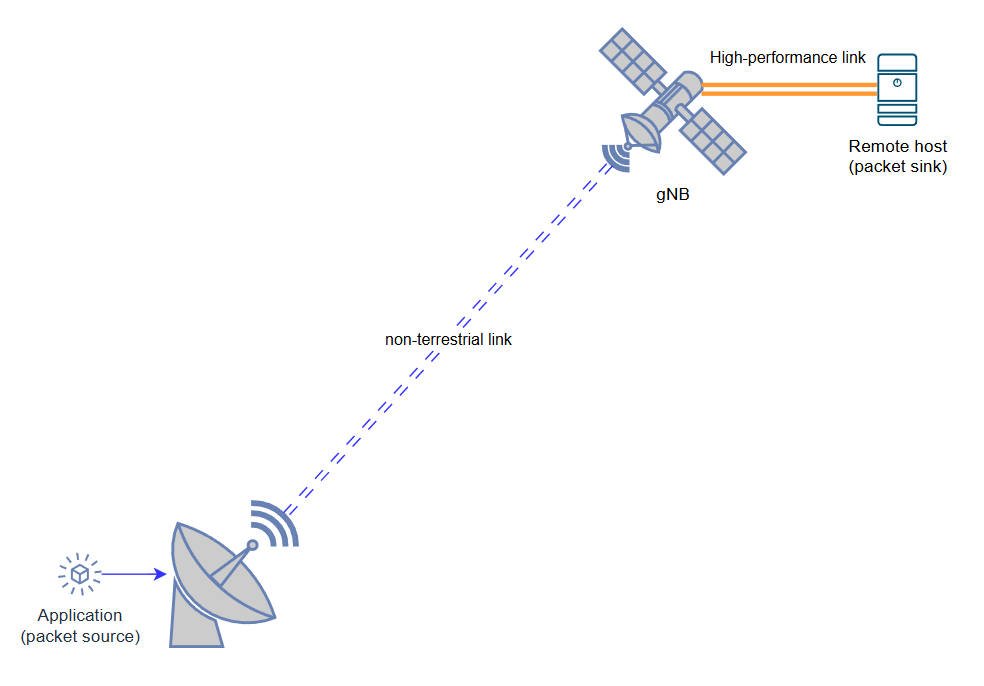
\includegraphics[width=0.8\textwidth]{res/sim-scenario.png}
    \caption{Network simulation scenario}
    \label{fig:sim-scenario}
\end{figure}

The simple network setup is depicted in Fig. \ref{fig:sim-scenario} and it consists of the following elements:
\begin{itemize}
    \item \textbf{Packet source}: application installed on the user equipment that generates packets with a specified periodicity. Both the generation rate and the packets' size can be varied by acting on their respective parameters. All the other variables that can be controlled are listed in the table \ref{tab:params}.
    \item \textbf{UE antenna}: the transmission of data is performed by mean of a \ac{vSAT} antenna placed at the \ac{UE} side. The main parameters of such antenna are found in the table \ref{tab:ue_params}.
    \item \textbf{Non-terrestrial link}: link connecting the \ac{UE} placed on the ground with the \ac{gNB}. This wireless link is characterized its propagation delay, bandwidth and frequency. However, since the aim of this work is to study the effects of propagation delay on the protocol suite, the bandwidth and frequency remained constant across all the simulations to better isolate the variables that could potentially cause problems. The list of parameters can be found in Table \ref{tab:link_params}.
    \item \textbf{g-NodeB}: the adopted approach is to incorporate the g-NodeB into the satellite payload, therefore adopting the configuration described in section \ref{sec:onboard-gnb}. This decision was made since the high one-way propagation delay is enough to cause some of the involved protocols to start malfunctioning. Adopting the bent-pipe configuration described in \ref{sec:bent-pipe-payload} would have resulted in effectively doubling the delay between \ac{UE} and \ac{gNB}. The satellite aperture antenna parameters follow the ones specified in the scenario named "10 DL" described in \cite{3gpp-tr-38.821}, and are listed in the table \ref{tab:sat_params}.
    \item \textbf{High performance link}: link connecting the g-NodeB to the packet sink. This is part of 5G core network, and it shall not be causing any additional problems, since that would be out of the scope of this work. This link was therefore meant to be as close as possible to an ideal one, with a capacity of 100Gb/s, a \ac{MTU} of 1500B and a delay of a single microsecond.
    \item \textbf{Remote host}: packet sink representing the destination node of all the packets generated at the \ac{UE}.
\end{itemize}

\begin{table}[ht]
    \begin{small}
    \begin{tabular}{l|ll}
    \textbf{Parameter name} & \textbf{Description}                       & \textbf{Default} \\ \hline
    enableNagle             & whether to enable Nagle's algorithm        & false            \\
    enableHarq              & whether to enable HARQ protocol            & false            \\
    numHarq                 & number of concurrent HARQ processes per UE & 16               \\
    harqTimeout             & timeout for HARQ processes                 & 100 ms           \\
    rrcIdeal                & use ideal RRC                              & false            \\
    tcpMinRto               & minimum TCP RTO                            & 200 ms           \\
    tcpBufSize              & TCP buffer size                            & 13107200 B       \\
    ipv4FrExpTimeout        & IPv4 fragment expiration timeout           & 200 ms           \\
    perr                    & target error probability for PHY packets   & 0.1              \\
    transportPrtcl          & whether to use UDP or TCP                  & UDP              \\
    numPackets              & max number of packets to be sent           & 2000             \\
    appStartTimeSec         & application start time                     & 0.5 s            \\
    appStopTimeSec          & application stop time                      & 5.5 s            \\
    simStopTimeSec          & simulation stop time                       & 6 s              \\
    packetSizeBytes         & application packets size                   & 200 B           
    \end{tabular}
    \end{small}
    \caption{Application and UE configuration parameters}
    \label{tab:params}
\end{table}



\begin{table}[ht]
    \begin{small}
    \begin{tabular}{l|ll}
    \textbf{Parameter name} & \textbf{Description}             & \textbf{Default} \\ \hline
    vsatAntennaGain         & gain of the vSat antenna         & 39.7 dB          \\
    vsatAntennaDiameter     & diameter of the vSat antenna     & 0.6 dB           \\
    vsatAntennaNoiseFigure  & noise figure of the vSat antenna & 1.2 dB          
    \end{tabular}
    \end{small}
    \caption{UE antenna parameters}
    \label{tab:ue_params}
\end{table}

\begin{table}[ht]
    \begin{small}
    \begin{tabular}{l|ll}
    \textbf{Parameter name} & \textbf{Description}                  & \textbf{Default} \\ \hline
    satEIRPDensity          & EIRP density of the satellite antenna & 40 dBW/MHz       \\
    satAntennaGain          & gain of the satellite antenna         & 58.5 dB          \\
    satAntennaDiameter      & diameter of the satellite antenna     & 5 m              \\
    distance                & orbiting altitude of the satellite    & -1 km           
    \end{tabular}
    \end{small}
    \caption{Satellite antenna parameters}
    \label{tab:sat_params}
\end{table}

\begin{table}[ht]
    \begin{small}
    \begin{tabular}{l|ll}
    \textbf{Parameter name} & \textbf{Description} & \textbf{Default} \\ \hline
    propDelay               & propagation delay    & 6 ms             \\
    frequency               & carrier frequency    & 20E9 Hz          \\
    bandwidth               & link bandwidth       & 400E6 Hz        
    \end{tabular}
    \end{small}
    \caption{Non-terrestrial link parameters}
    \label{tab:link_params}
\end{table}


\section{5G scheduler}
As the name suggests, the main task of the scheduler is to allocate resources to the various connected users in the form of transmission and reception opportunities. In the \ac{NR} standard, the scheduling is dictated by the network and the \ac{UE} has to follow the provided indications \cite{5g-sched-sharetechnote}.

In the \ac{NR} standard, the scheduling process is similar to LTE, with the addition of some new factors and flexibility options. 

\subsection{Frame structure}
The scheduler divides time using four different entities: frames, subframes, slots and symbols. 5G \ac{NR} frame structure is defined in \ac{3GPP} TS 38.211 \cite{3gpp-ts-38.211}. 

Frames always have a duration of 10 ms, while subframes are 1 ms long. Slots and symbols have variable lengths instead, based on the value of a parameter called numerology and represented with the letter $\mu$. Regardless of its time duration, each slot always contain 14 \ac{OFDM} symbols. \cite{gaussianwaves-frame}. 

The $\mu$ parameter can assume integer values in the range $\left[0, 4\right]$, and its value affects the subcarrier spacing and bandwidth, as well as the slot and the symbol durations. Table \ref{tab:mus} contains the values for each supported value of $\mu$ \cite{gaussianwaves-frame}.

\begin{table}[ht]
    \begin{tabular}{l|lllll}
    \textbf{$\mu$} & \textbf{\begin{tabular}[c]{@{}l@{}}Subcarrier spacing\\ $\Delta f = 2^\mu \times 15 \text{kHz}$\end{tabular}} & \textbf{\begin{tabular}[c]{@{}l@{}}Resource block\\ bandwidth\\ $\Delta f \times 12$\end{tabular}} & \textbf{\begin{tabular}[c]{@{}l@{}}Slots per\\ frame\end{tabular}} & \textbf{\begin{tabular}[c]{@{}l@{}}Slot\\ duration\end{tabular}} & \textbf{\begin{tabular}[c]{@{}l@{}}Symbol\\ duration\end{tabular}} \\ \hline
    \textbf{0}  & 15 kHz                                                                        & 180 kHz                                                                               & 10                                                                 & 1 ms                                                             & 71.43 $\mu \text{s}$                                                              \\
    \textbf{1}  & 30 kHz                                                                        & 360 kHz                                                                               & 20                                                                 & 500 $\mu \text{s}$                                                          & 35.71 $\mu \text{s}$                                                              \\
    \textbf{2}  & 60 kHz                                                                        & 720 kHz                                                                               & 40                                                                 & 250 $\mu \text{s}$                                                             & 17.86 $\mu \text{s}$                                                             \\
    \textbf{3}  & 120 kHz                                                                       & 1.44 MHz                                                                              & 80                                                                 & 125 $\mu \text{s}$                                                             & 8.93 $\mu \text{s}$                                                              \\
    \textbf{4}  & 240 kHz                                                                       & 2.88 MHz                                                                              & 160                                                                & 62.5 $\mu \text{s}$                                                            & 4.46 $\mu \text{s}$                                                             
    \end{tabular}
    \caption{Supported numerologies}
    \label{tab:mus}
    \end{table}

Figures \ref{fig:frame1} and \ref{fig:frame2} show the difference in radio frame configuration for $\mu = 0$ and $\mu = 1$. In the first case, each subframe has exactly one slot, while in the second case each subframe contains two slots, the subcarrier bandwidth is doubled and the duration of each symbol halved.

\begin{figure}[ht]
    \centering
    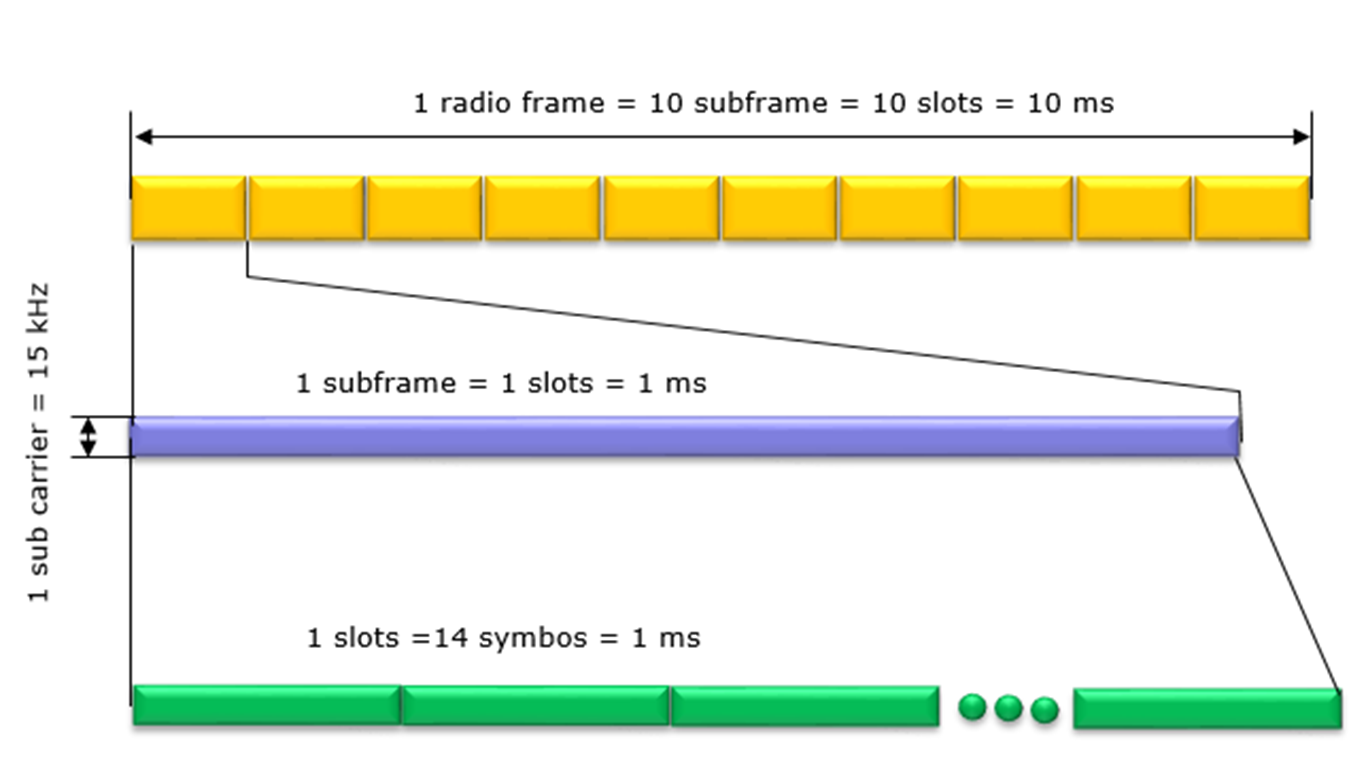
\includegraphics[width=0.8\textwidth]{res/frame-1.png}
    \caption{Radio frame structure for $\mu=0$ \cite{frame-5gnet}}
    \label{fig:frame1}
\end{figure}

\begin{figure}[ht]
    \centering
    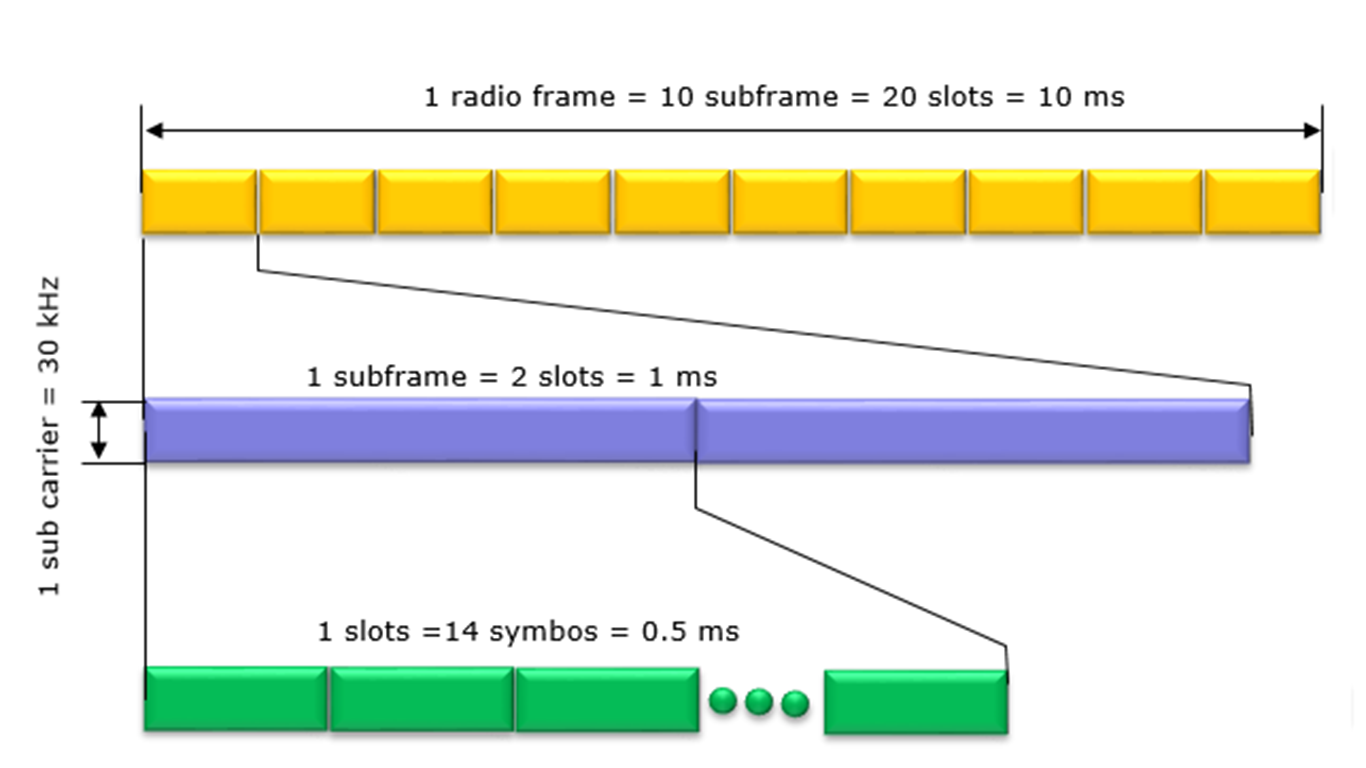
\includegraphics[width=0.8\textwidth]{res/frame-2.png}
    \caption{Radio frame structure for $\mu=1$ \cite{frame-5gnet}}
    \label{fig:frame2}
\end{figure}

\subsection{Dedicated configuration}
Differently from LTE, where a predefined pattern was in place when allocating downlink and uplink slots in a radio frame, in \ac{NR} this is done much more flexibly using a plethora of parameters such as the periodicity of UL and DL transmissions, the number of consecutive DL and UL slots and symbols at the beginning of each pattern and more \cite{5g-sched-sharetechnote}

In LTE, once a subframe is flagged as either UL or DL, all of its symbols are used for the allocated purpose, while \ac{NR} enables symbol-level scheduling, meaning that we don't need to use every symbol within a slot, and each slot can be further divided in groups of symbols reserved for UL and DL. The term slot format indicates how each symbol within a slot is used \cite{frame-5gnet}. 


\subsection{Propagation delay and differential delay}
\paragraph{}The important key concept is that the scheduler shall account for the propagation delay. While in terrestrial communications a guard period of six symbols when switching from downlink communications to uplink communications is sufficient to account for the delay in a few km-radius cell, and timing advance commands can account for the different propagation delays experienced by users located in the center of the cell and users located in the cell edge \cite{gsma-5g-tdd-sync}, the same cannot be said for non-terrestrial use cases, where the distances that come into play are much longer, therefore delays are higher.

Consider the case depicted in Figure \ref{fig:diff-delay} from \cite{preamble-detection-chougrani}. For a \ac{LEO} satellite orbiting at 600Km, cell diameter of 82Km and elevation angle of 45°, the maximum differential round-trip delay of UE2 with respect to UE1 is of $370\mu s$ \cite{preamble-detection-chougrani}. On the other hand, a 3km-radius cell experiences a maximum round-trip differential delay of $2*\text{radius}/c \approx 10\mu s$

\begin{figure}[ht]
    \centering
    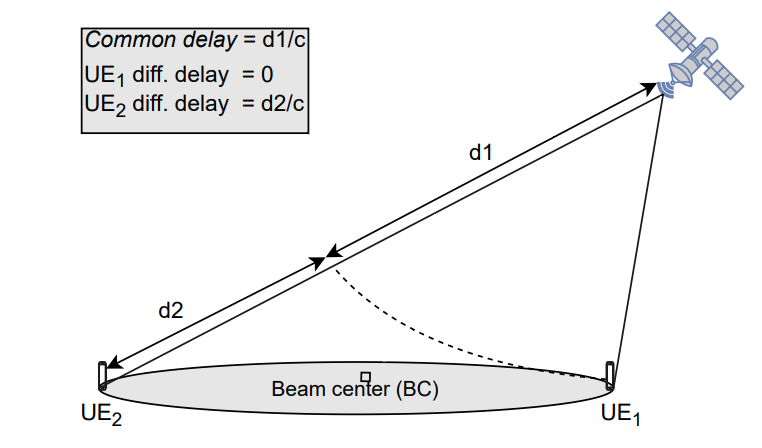
\includegraphics[width=0.8\textwidth]{res/diff-delay.png}
    \caption{Differential delay for \ac{NTN}, courtesy of \cite{preamble-detection-chougrani}.}
    \label{fig:diff-delay}
\end{figure}


\section{Accounting for propagation delay in scheduling}
\label{sec:pd-sched-acc}

\subsection{Problem description}
\label{ss:propdelay-problem-desc}
\paragraph{}
The first encountered problem while implementing a non-terrestrial communication scenario in the simulator was the inability of the scheduler to account for the propagation delay when allocating radio resources to the connected user equipment on the ground.

The implementation of the 5G scheduler in ns-3 is designed to allocate resources less than a single subframe in advance, and since each subframe has a duration time of 1ms, the resource grant was already expired by the time it was able to reach the \ac{UE}, since it was referring to a past subframe.

\paragraph{Example} Consider a scenario with a propagation delay $\tau_p$ of 6ms, corresponding to a satellite at an altitude of 1800 km. The \ac{UE} sends a request for uplink resources at time $t_0$ since it has some data to send. In the standard scheduler implementation, assuming an ideal transmission, the \ac{gNB} would receive such request at $t_0+\tau_p=6\textit{ms}$. Provided that other transmissions have not been scheduled yet, the \ac{gNB} grants the \ac{UE} the possibility to transmit in the following subframe, which will start after 1ms at $t_0+\tau_p+t_{\textit{SF}}=7\textit{ms}$. The grant that allows the \ac{UE} to transmit at $t=7\textit{ms}$ is ideally transmitted by the \ac{gNB} as soon as it receives the request, therefore at $t=6\textit{ms}$. However, this grant will reach the \ac{UE} only after another propagation delay, at $t_0+2\tau_p=12\textit{ms}$, when the transmission opportunity would already have expired.

\subsection{Implemented solution}
\label{ss:propdelay-problem-sol}
The implemented solution assumes that the scheduler has knowledge of an estimation of the propagation delay, that can be obtained through the use of probe signals and basing on previously measured values. This is a reasonable assumption since systems such as GPS already rely on a precise estimation of the delay between the user on the ground and the satellite.

The scheduling then proceeds as normal with the only difference being that the information regarding the propagation delay is used to postpone the allocated symbols. 

\paragraph{Example} Consider a scenario with propagation delay $\tau_p$ of 5 slots (roughly 1,2ms). The new implementation of the scheduler accounts for the propagation delay by allocating the first available slot after $\tau_p$, so the time for the grant to reach the \ac{UE} is accounted for, and the \ac{gNB} marks the slot after $2\tau_p$ as reserved.

The last part of reserving a different slot is not as immediate. However, this mechanism needs to be in place because of the behavior depicted in Figure \ref{fig:scheduler-allocations-pd} and hereby detailed. In this scenario, the numerology $\mu$ is 2, therefore each subframe contains 4 slots.


\begin{itemize}
    \item \ac{UE} sends the scheduling request to \ac{gNB} at frame 1, subframe 0, slot 0.
    \item The \ac{SR} reaches the \ac{gNB} after $1\tau_p$ of 5 slots and the \ac{UE} is scheduled to transmit at frame 1, subframe 2, slot 2 since there is some noticeable propagation delay.
    \item The \ac{SR} reaches the \ac{UE} at frame 1, subframe 2, slot 2, and the \ac{UE} can transmit right away.
    \item The packet reaches the \ac{gNB} after another $\tau_p$, hence the base station needs to know that it cannot schedule other transmissions to take place in this slot, otherwise interference and collisions may arise.
\end{itemize}

\begin{figure}[ht]
    \centering
    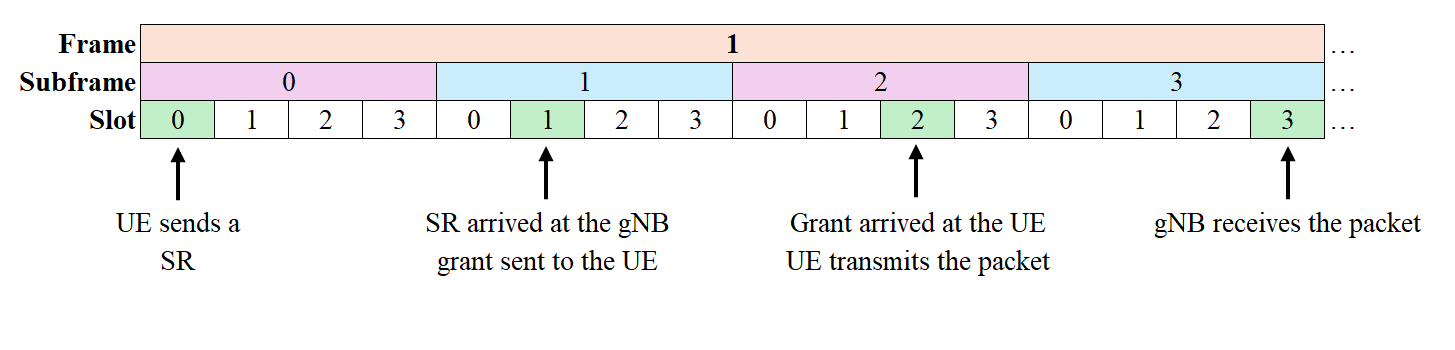
\includegraphics[width=0.9\textwidth]{res/scheduler-allocation-pd.png}
    \caption{Difference between allocated slot and gNB reception}
    \label{fig:scheduler-allocations-pd}
\end{figure}

\paragraph{ns-3 implementation}
This solution has been implemented as a modification to the classes \texttt{MmWaveFlexTtiMacScheduler} and \texttt{MmWaveEnbPhy}, that now account for delayed responses of previously scheduled transmissions when allocating new slots.

The classes \texttt{MmWaveUePhy} and \texttt{MmWavePhy} have also been modified to allow access to the propagation delay parameter of the physical channel.

\section{BSR timer}
\label{sec:bsr-timer}
After implementing the solution discussed in the previous point in the ns-3 network simulator, allowing the communication to take place, some other irregularities were found regarding the periodic \ac{BSR} timer, as described in the following. 

\subsection{Problem description}

\paragraph{Reduced latency}

Figure \ref{fig:lat-saw} shows a rather peculiar trend regarding latency. The expected result was a linear increase in latency with a slope of 3, where every packet arrived at the destination after three times the propagation delays. The reasoning behind this expectation was that every packet generated by the application should have triggered a scheduling request received by the \ac{gNB} after $\tau_p$, a grant to be emitted requiring another $\tau_p$ to reach the \ac{UE}, and finally the transmission to be received by the \ac{gNB} after the third propagation delay (with the assumption of ideal transmission).

The observed pattern did not match any of the expectations. The output obtained from the simulation campaign showed a nonlinear saw tooth behavior presenting values that consistently stayed under the expected $3\tau_p$ threshold value, shown in green in Fig. \ref{fig:lat-saw}.

\begin{figure}[ht]
    \centering
    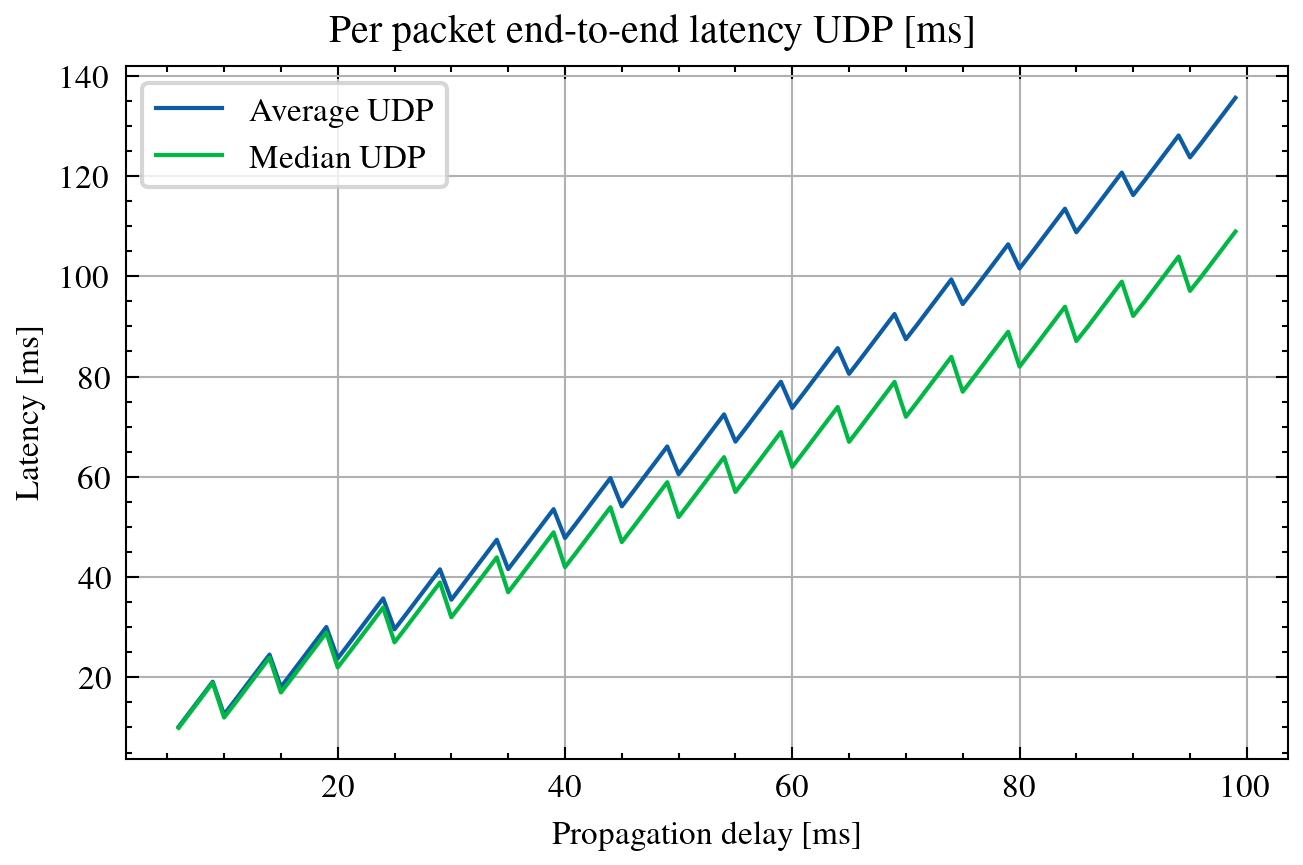
\includegraphics[width=0.8\textwidth]{res/lat-udp-saw.png}
    \caption{E2E latency vs. propagation delay with periodic \ac{BSR}}
    \label{fig:lat-saw}
\end{figure}

\paragraph{Periodic buffer status reports} Further investigation on the subject allowed identifying numerous buffer status reports sent from the \ac{UE} to the \ac{gNB} at regular intervals of 10ms, even when no new packets were produced by the application.

Buffer status reports are messages that the \ac{UE} uses to communicate to the \ac{gNB} the status of its transmission buffer. Every new packet arriving to the transmission buffer of the \ac{UE} changes its status and a new \ac{BSR} is sent, containing information such as the number of queued packets and their size. Upon reception, the \ac{gNB} can grant the \ac{UE} some resources to transmit part or all of the contents of its buffer. Each \ac{BSR} is therefore interpreted as a \ac{SR}.

This behavior happens because the implementation of 5G \ac{MAC} layer includes a periodic \ac{BSR} that the \ac{UE} sends to the \ac{gNB} as long as the transmission buffer contains some pending data.
The details of this mechanism are documented in Section 5.4.5 of the standard \cite{etsi-mac-specification}, where it is also stated that the default interval between those periodic \ac{BSR} is of 10ms.

This characteristic was meant to act as a safeguard against lost scheduling requests, and does not account for the propagation delay at all. The \ac{UE} therefore continues to send additional buffer status reports at regular 10ms intervals even though the previous ones were not lost, but still travelling towards the base station because of a (very long) in-fligh propagation delay.

\paragraph{}
Figure \ref{fig:diagram-wasted-capacity} illustrates this behavior. The arrival at the \ac{UE}'s application buffer of packet p1 at time $t=0$ triggers the transmission of a first \ac{SR}. Since the hereby depicted scenario has a propagation delay of 20ms, the \ac{SR} will arrive at the g-NodeB at time 20ms. However, the \ac{BSR} timer expires at $t=10\text{ms}$ by default, so during a single round-trip time the \ac{BSR} is repeated four times. The green arrows marked with a capital G denote all the grants issued to the \ac{UE}. Only one of the four depicted will actually be used by the \ac{UE} for the intended packet, effectively wasting three out of four transmission opportunities that could have been allocated to other users waiting to transmit.

\begin{figure}[ht]
    \centering
    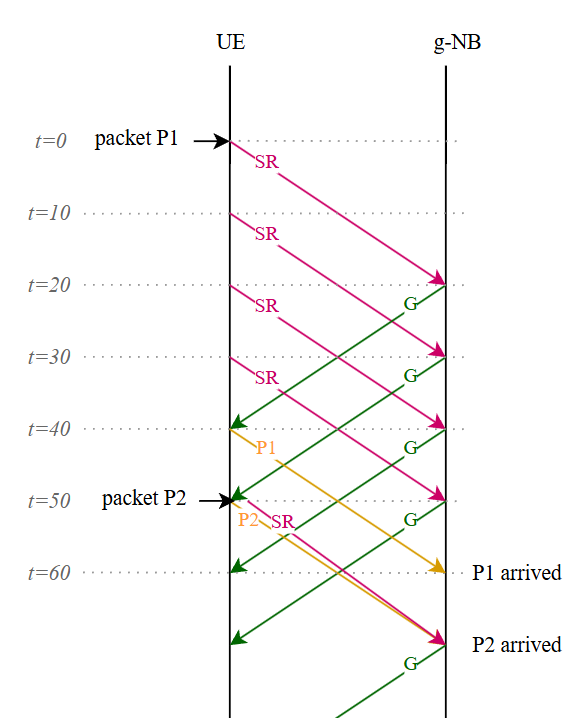
\includegraphics[width=0.5\textwidth]{res/diagram-wasted-grants.png}
    \caption{Packet diagram with periodic \ac{BSR}}
    \label{fig:diagram-wasted-capacity}
\end{figure}

The reduction in latency was observed because newly arrived packets could, in certain situations, make use of the resource grants that were meant for the previous packets but have yet to arrive at the \ac{UE}. Consider the arrival of another packet (P2) at the\ac{UE}'s application buffer. in figure \ref{fig:diagram-wasted-capacity}. It triggers another \ac{SR}, but a grant (originally intended for and trigger by P1) is received immediately after, therefore allowing for an immediate transmission of P2, which will experience a latency of only a single propagation delay. This instantaneous grant is nothing but the result of the previous \ac{SR} storm originated from the \ac{UE} itself.

While this can present some beneficial aspects such as the reduced overall latency, it originates from a behavior that is outside the original design intentions. Moreover, this approach is particularly greedy, leading to wasted capacity.

\subsection{Implemented solution}

After the successful identification and characterization of the problem, the  solution consisted of the implementation of a simple adaptive algorithm that would dynamically set the \ac{BSR} timer to a value of twice the propagation delay plus a constant of 4ms that accounts for the processing times as well as any possible delay. The constant was chosen accounting for the characteristics of the link, the packets transmission times as well as processing times.

\paragraph{ns-3 implementation}
Modifications were made to the \texttt{LteRlcUm} class to expose the buffer status report timer parameter using the ns-3 attribute framework, therefore permitting its dynamic adjustment based on the propagation delay. 

This allowed the simulation manager software to test different values of the \ac{BSR} timer, as well as a more standardized way of setting its value without changes to the source code. Figure \ref{fig:lat-improved} shows the result of our implementation. Latency now closely follows the expected results, only presenting a marginal increase due to the non-null transmission and processing times.

\begin{figure}[ht]
    \centering
    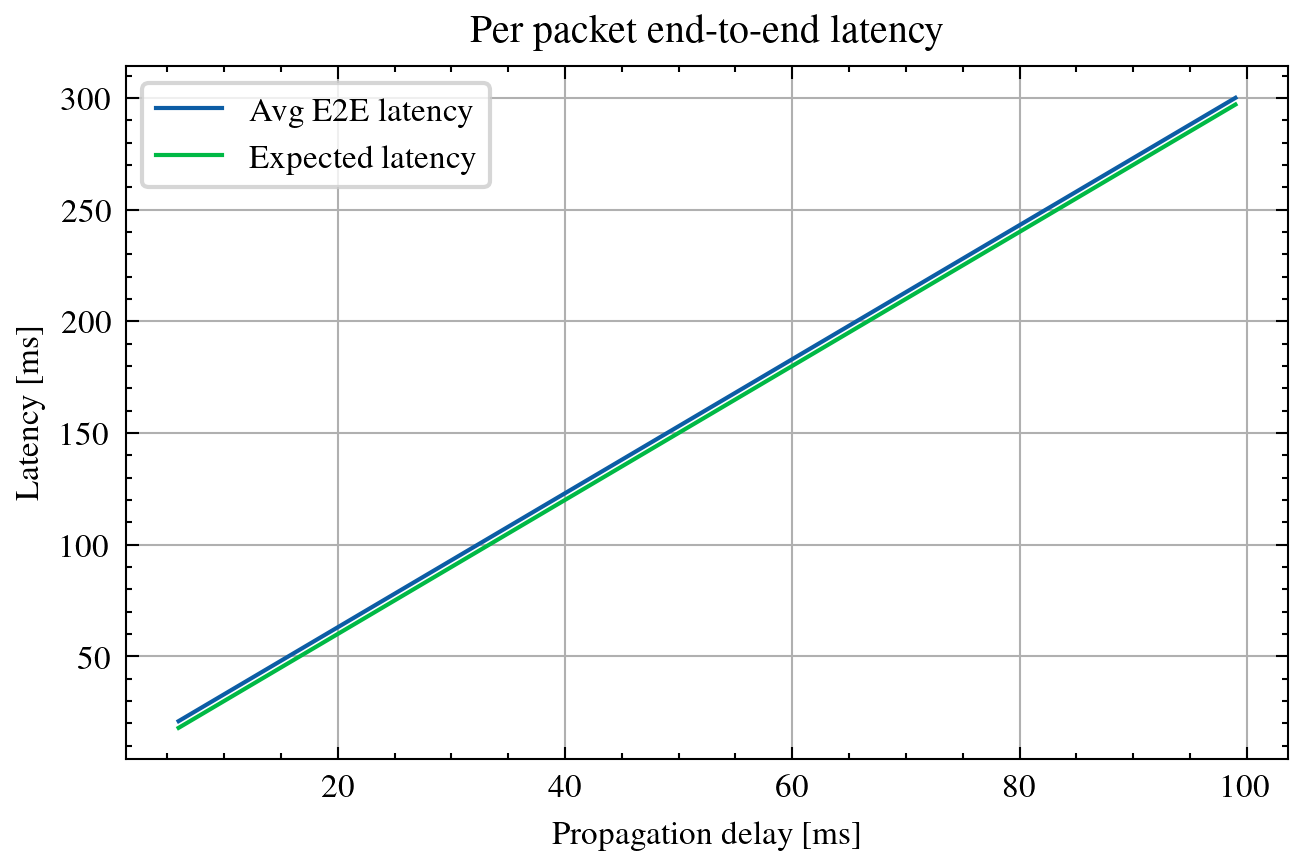
\includegraphics[width=0.8\textwidth]{res/lat_sched_after.png}
    \caption{E2E latency vs. propagation delay with implemented solution}
    \label{fig:lat-improved}
\end{figure}


\paragraph{Area of potential improvement}
The implementation of the aforementioned solution, however, while working as intended, had the expected but unwelcomed effect of increasing the overall latency of the system, since all the additional grants required by previous packets that newly generated ones could exploit were no longer available.

This unexpected problematic behavior of wasted transmission opportunities accidentally also unveiled the potential of preemptively transmitting additional scheduling requests, so that future packets could be sent with a lower latency.

If implemented correctly, the \ac{UE} could adopt a predictive approach towards its traffic needs for the near future basing its estimates on the type of application, and send the \ac{gNB} scheduling requests for packets that have yet to be generated.

\section{Inflated BSR}
\label{sec:inf-bsr}

\subsection{Problem description}
Another problem occurred when the interval between the packets generated by the application, i.e. the packets interarrival time, was smaller than a single round-trip time. 

\paragraph{}
The arrival of each packet automatically triggers the transmission of a scheduling request by the \ac{UE}. However, each request is made for the whole transmission buffer. This causes a problem when many packets arrive before the \ac{gNB} has the chance to respond with the appropriate resource grant.

Referring to Figure \ref{fig:inflated-bsr-diag}, we can see that the arrival of P1 in the transmission buffer of the \ac{UE} triggers the transmission of a \ac{SR} for a single packet. The second packet P2 arriving after 10ms triggers another request, however this second request is cumulatively made for the full buffer length, regardless of the fact that the first \ac{SR} is still pending. This is denoted by the writing "SRx2". Packets P3 and P4 behave in the same way, triggering requests for the allocation of three and four additional packets respectively.

Finally, the grants start arriving at the \ac{UE}. The first 1-packet grant allows for the transmission of P1, while the second grant, requested for two packets, allows for the transmission of packets P2 and P3. The third grant, which corresponds to a previous request for 3 packets and could therefore allow the transmission of 3 packets, can now only be used by P4, wasting 2/3 of its potential capacity. 

The last grant, that would allow the \ac{UE} to transmit 4 consecutive packets, is completely wasted since the send buffer is now empty.

\begin{figure}[ht]
    \centering
    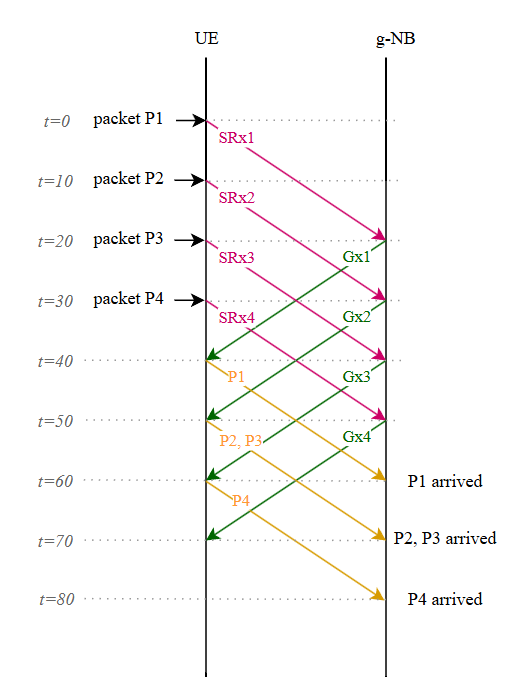
\includegraphics[width=0.5\textwidth]{res/diagram-inflated-bsr.png}
    \caption{Packet diagram for interarrival times smaller than propagation delay}
    \label{fig:inflated-bsr-diag}
\end{figure}
\begin{figure}[ht!]
    \centering
    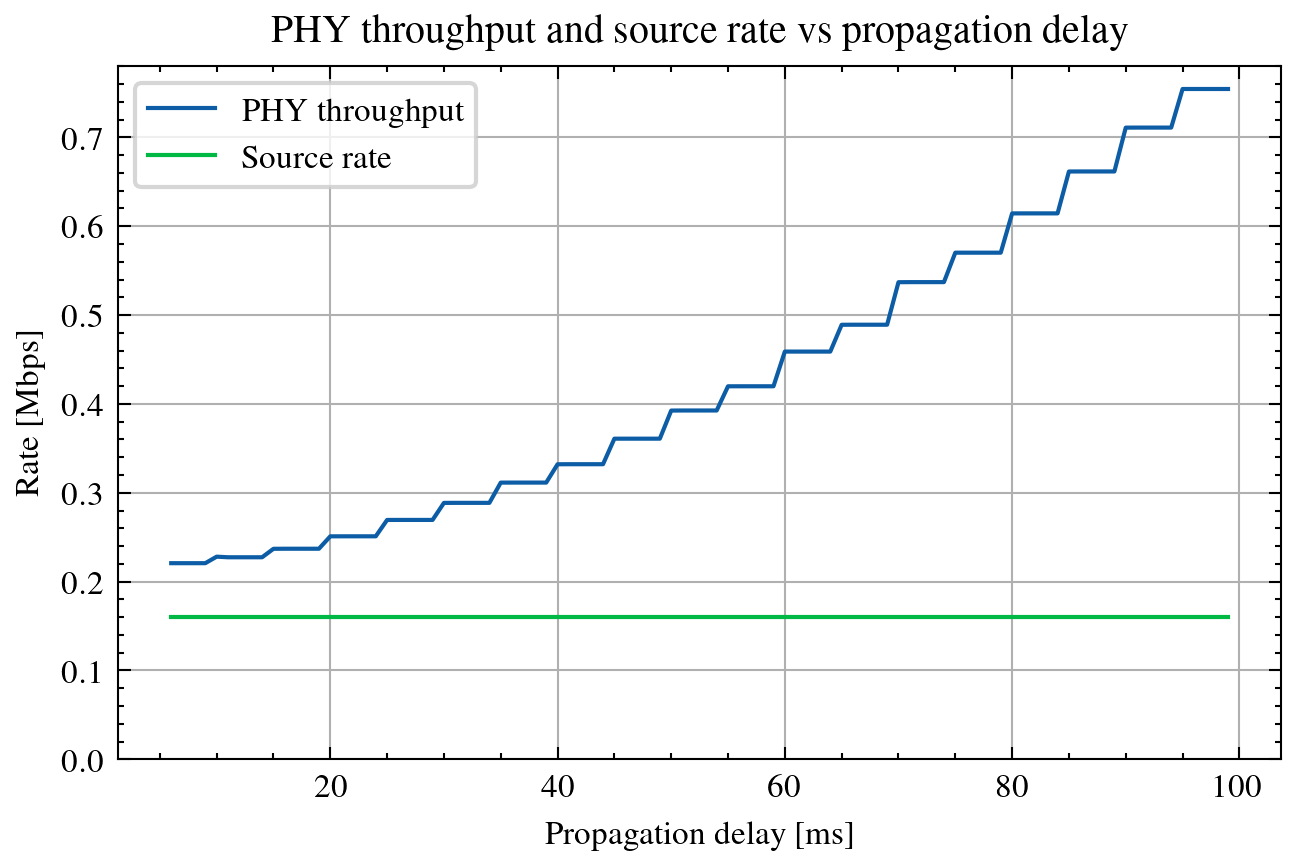
\includegraphics[width=0.8\textwidth]{res/phy-thr-udp-runaway-new.png}
    \caption{Physical throughput and application source rate vs. propagation delay with inflated requests}
    \label{fig:phy-thr-runaway}
\end{figure}
\paragraph{Repercussions}
The described behavior caused the physical throughput to be significantly higher than the application source rate, since the physical throughput metric counts all the capacity assigned to the \ac{UE}, even though part of it might be just padding. Figure \ref{fig:phy-thr-runaway} shows the observed physical throughput for a constant source rate of 160Kb/s. The area between the two lines indicates that a lot of radio resources are being wasted to transmit few data. All the unused space in the grants that the \ac{UE} receives is filled with padding, that counts as physical throughput but is useless at the higher levels. The growing trend when the propagation delay increases happens because the \ac{SR} and grants take more time to arrive at their destinations, and the \ac{UE} keeps sending inflated \ac{BSR}s for more time, further contributing to waste more resources.



\subsection{Implemented solution}

Various different approaches could be undertaken in order to tackle this problem. Nonetheless, a comprehensive study detailing upsides and downsides of each of them is outside the scope of this thesis. 

The implemented solution consists of a modification to the \ac{SR} algorithm that limits the requests to only account for the newly received data, therefore disabling the cumulative behavior. If a packet is already in the buffer when a new one arrives, the scheduling request only asks the size of the second packet to be allocated.
\begin{figure}[ht]
    \centering
    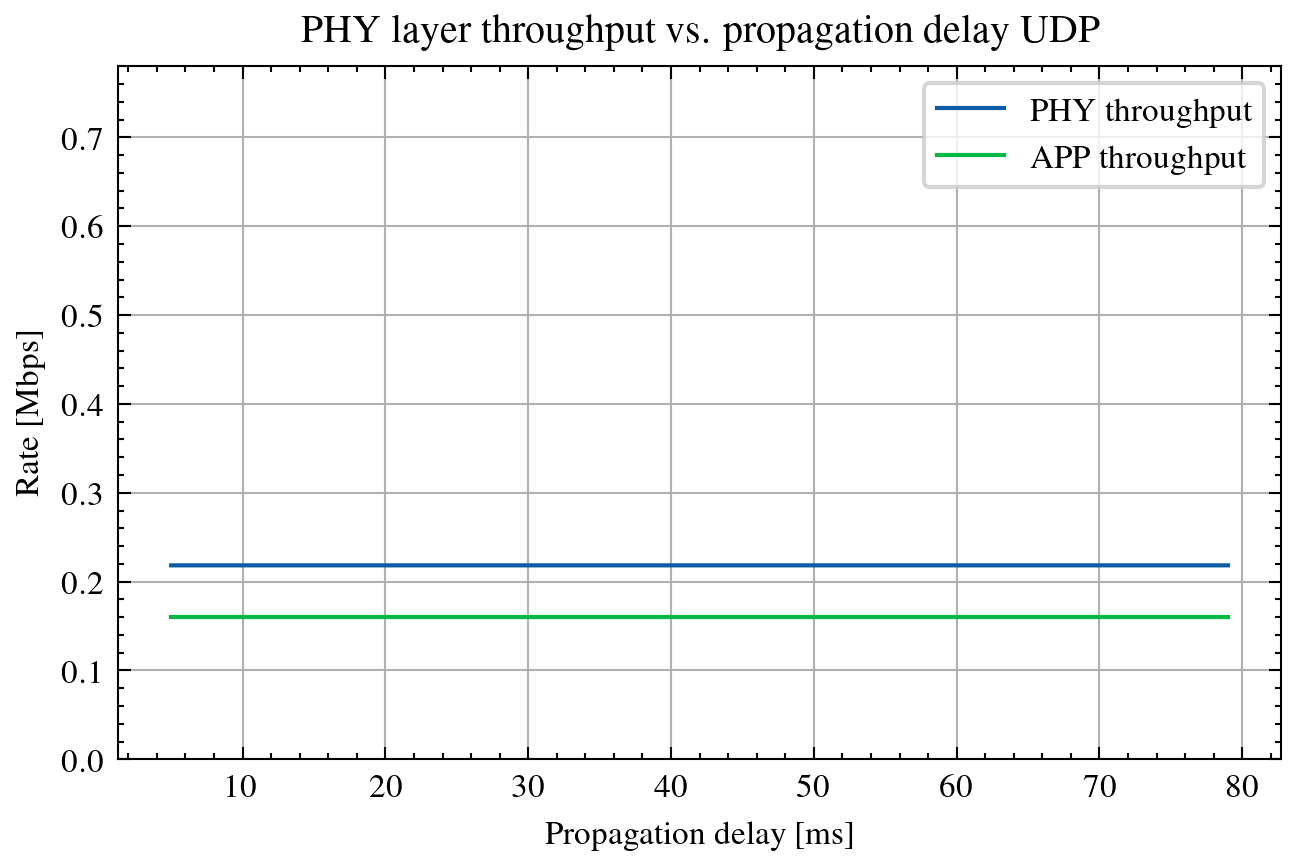
\includegraphics[width=0.8\textwidth]{res/phy_thr_new.png}
    \caption{PHY throughput vs. propagation delay with implemented solution}
    \label{fig:phy-thr-after}
\end{figure}

\begin{figure}[ht!]
    \centering
    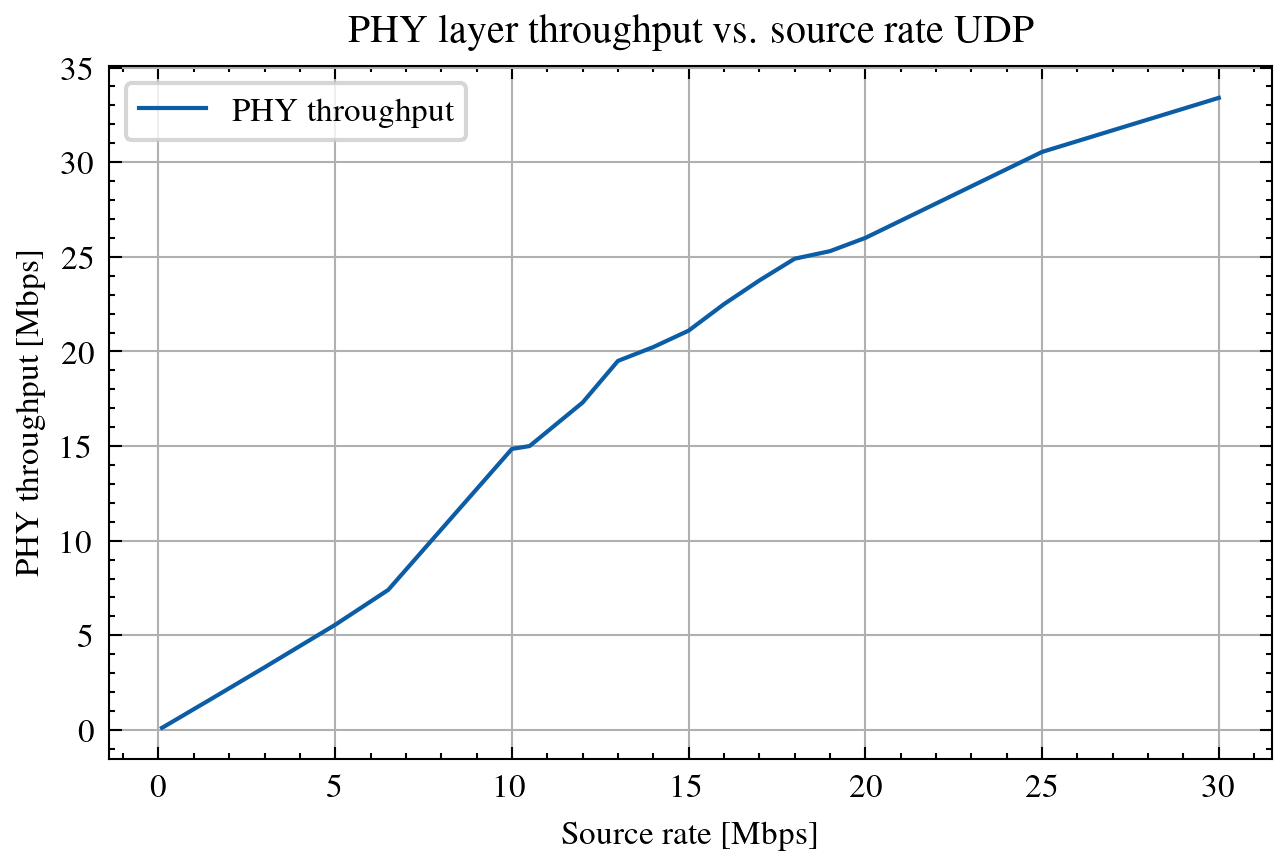
\includegraphics[width=0.8\textwidth]{res/phy_vs_sr.png}
    \caption{Physical throughput vs. source rate}
    \label{fig:phy-vs-sr}
\end{figure}
The effectiveness of the implemented solution can be seen in Figure \ref{fig:phy-thr-after}, showing that the physical layer throughput remains constant as the propagation delay increases, as reasonably expected since the source rate is constant throughout the simulation.



Finally, Figure \ref{fig:phy-vs-sr} shows the behavior of the physical throughput as the application source rate increases. Note that the application rate is always smaller than the physical throughput. This happens because the \ac{TB} that the \ac{gNB} assigns to the \ac{UE} have dimensions that can only be integer multiples of the size of an OFDM symbol, therefore each \ac{TB} can be slightly larger than the actual application-level packet. Furthermore,physical throughput also accounts for protocol overheads, otherwise discarded in the computation of the application source rate.

\paragraph{ns-3 implementation}
The method responsible for the cumulative buffer status reports is \texttt{DoReportBufferStatus()} in the \texttt{LteRlcUm} class, therefore it was modified to only account for the newly arrived data when sending a \ac{SR}.


\section{Reordering timer}
\label{sec:reord-timer}

\subsection{Problem description}
\paragraph{Fragmentation}
The packets interarrival times are not necessarily multiples of the propagation delay, and the resources that the g-NodeB grants to the \ac{UE} are usually a few bytes larger than the packet size. This happens because, even though 5G scheduling can be done on a much finer granularity than 4G scheduling, the base station still cannot grant values that are smaller than a single symbol, so the general rule is to allocate the minimum number of symbols whose cumulative size is greater or equal to the requested allowance.

This misalignment between packet size and transmission opportunities allows for packets to be split in smaller pieces. If two packets of 200B each are waiting in the buffer to be transmitted, and a resource grant for 220B arrives at the \ac{UE}, the first packet can be completely transmitted, but it would be wasteful not to use also the 20 additional bytes that were granted, so the second packet is split and only its first bytes are transmitted. The remaining ones will wait for the next opportunity.

\paragraph{PDCP}
The detailed implementation of the \ac{PDCP} layer can be found in the \ac{3GPP} technical specification \cite{pdcp-spec-3gpp}, while the diagram describing its functionality has been reported in Figure \ref{fig:pdcp-functionalities}. This layer offers reordering services by employing a sequence number, integrity protection and ciphering if the packet in question is associated to a \ac{PDCP} \ac{SDU}, and duplication and routing when operating split bearers.

\begin{figure}[ht]
    \centering
    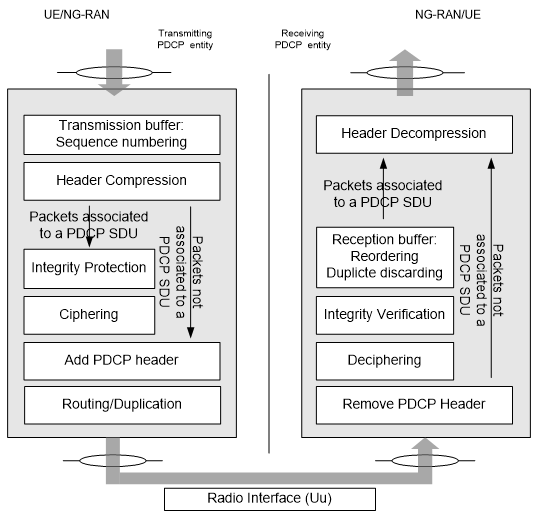
\includegraphics[width=0.7\textwidth]{res/pdcp-functionality.png}
    \caption{PDCP diagram \cite{pdcp-spec-3gpp}}
    \label{fig:pdcp-functionalities}
\end{figure}

The observed problem, as the propagation delay increases, is related to an expiring timer when reassembling the packets at the \ac{PDCP} layer. The so-called reordering timer (t-reordering), which despite the name also affects the recomposition of fragmented packets, is not configured for the use in a non-terrestrial scenario, and it regularly expires due to the long propagation delay before the second half of the packet managed to arrive, leading to the discard of otherwise good packets.

This re-ordering functionality of \ac{PDCP} layer is in place to ensure a sequential delivery of packets to the upper layers. In case of missing packets, the approach is to wait until either the packets arrive or the reordering timer expires \cite{efficient-reassembly-pdcp}. It was observed that this timer also started when the \ac{PDCP} layer was waiting for the arrival of the second part of a fragmented packet. However, due to the high propagation delay, the second half of the packet did not arrive before the timer expiration, leading to the packet being discarded.

Should the reordering timer be set too high, it may cause additional latency, and, if set too low, it might cause many packets to be discarded, as in the case that was hereby simulated.


\subsection{Implemented solution}
Since the use of timers always bears trade-offs depending on their value, in this case either being a higher latency or a higher packet discard ratio, there can not be a one-fits-all approach: the differences in propagation delays between satellites orbiting at different altitudes are so drastic that the implementation of a single default value would lead to suboptimal performances in every possible scenario. 

The class \texttt{LteRlcUm} was therefore modified to expose the \texttt{ReorderingTimer} parameter, allowing to easily set its value using the ns-3 attribute framework, similarly to the approach undertaken while solving the previous problem. This in turn permitted to set the timer to the value of the propagation delay plus a small constant accounting for processing delays for each simulator run.